
%(BEGIN_QUESTION)
% Copyright 2006, Tony R. Kuphaldt, released under the Creative Commons Attribution License (v 1.0)
% This means you may do almost anything with this work of mine, so long as you give me proper credit

Explain how the gain adjustment works in this pneumatic proportional controller mechanism:

$$\includegraphics[width=15.5cm]{i01482x01.eps}$$

By moving the ``gain adjust rod'' up and down, the controller gain may be varied.  Identify which direction of motion will result in {\it more} gain.

\vskip 20pt \vbox{\hrule \hbox{\strut \vrule{} {\bf Suggestions for Socratic discussion} \vrule} \hrule}

\begin{itemize}
\item{} Identify at least one advantage this method of gain adjustment enjoys over other methods of gain adjustment you have seen in pneumatic controller mechanisms.
\item{} Suppose this pneumatic control mechanism were augmented with an {\it amplifying relay} to improve its performance.  Where exactly would the new relay be placed within the mechanism?
\item{} How would this controller mechanism act if the orifice were relocated to a position between the output tube and the nozzle, rather than between the air supply and the output tube where it should be?
\item{} Sketch an electronic opamp circuit with an adjustable gain that works analogously to this pneumatic controller mechanism.
\end{itemize}

\underbar{file i01482}
%(END_QUESTION)





%(BEGIN_ANSWER)

Hint: the pneumatic {\it pilot} mechanism is analogous to an electrical potentiometer when wired as a voltage divider.

\vskip 10pt

To see an electrical analogue of this mechanism, sketch a negative-feedback opamp circuit where the inverting input of the opamp receives a fraction of the output voltage through a potentiometer.

%(END_ANSWER)





%(BEGIN_NOTES)

Moving the rod {\it down} results in the least amount of output pressure fed back to the bellows, increasing the gain of the controller.  This is similar to the feedback network in an operational amplifier circuit, where feeding back a smaller proportion of the output signal forces that output signal to exhibit a greater change that it would otherwise (i.e. a larger over-all gain).

\vskip 10pt

This controller design is based loosely on the Fisher ``Multi-Trol,'' using the same gain adjustment mechanism and the same motion-balance arrangement.

\vskip 10pt

By using variable pneumatic signal feedback to control the gain of this mechanism, the potential for {\it remote gain adjustment} becomes possible.








\vfil \eject

\noindent
{\bf Summary Quiz:}

In order to increase the {\it gain} of this controller, one must:

$$\includegraphics[width=15.5cm]{i01482x02.eps}$$

\begin{itemize}
\item{} Move the nozzle closer to the beam (flapper)
\vskip 5pt 
\item{} Move the plug of the pilot valve in a downward direction
\vskip 5pt 
\item{} Increase the compressed air supply pressure
\vskip 5pt 
\item{} Decrease the compressed air supply pressure 
\vskip 5pt 
\item{} Move the plug of the pilot valve in an upward direction
\vskip 5pt 
\item{} Move the nozzle further away from the beam (flapper) 
\end{itemize}


%INDEX% Control, proportional: pneumatic motion-balance controller

%(END_NOTES)


